\documentclass[a4paper,10pt]{article}
\usepackage[pdftex]{color,graphicx}
\usepackage[pdftex, bookmarks, colorlinks]{hyperref}
\usepackage{longtable}
\addtolength{\textheight}{2cm}
\addtolength{\textwidth}{2cm}
\addtolength{\hoffset}{-1cm}
\addtolength{\voffset}{-3cm}

%opening
\title{Genotyping}
% \author{Rong Jiang, Yu Huang}

\begin{document}

\maketitle

\begin{abstract}

\end{abstract}

\tableofcontents

\section{Genotyping}
The genotype calls are the foundation for all the following work. The accuracy of genotype calls has a fundamental impact on all the analyses, results and conclusions reached. We took great care to ensure we get the best calls possible.

The whole genotyping pipeline consists of running a modified Oligo package~\cite{Carvalho2007}, detailed in section~\ref{Oligo_calling}, filtering the dataset in several steps to remove arrays and SNPs deemed of bad quality, imputation, etc.

We did not solely rely on Oligo because of the limited 20-accession dataset~\cite{Clark2007a} used in training Oligo. Oligo occassionally assigns high probability to the calls in certain arrays while QC with previous datasets shows very high mismatch rates. After excluding the possibility of accession ID mis-labeling, we find out it's their peculiar intensity distribution, which is quite different from the arrays used in training.

\subsection{Platform}
The SNP genotyping was performed with the Affymetrix 250K SNP-tiling array (AtSNPtile1). One SNP-tiling array contains probe sets for 248,584 pre-selected SNPs and each SNP is represented by a probe set of four probes, i.e., combinations of two alleles and two strands (sense and anti-sense). Samples were processed at the microarray core facilities at the University of Chicago and Children Hospital of Los Angeles affiliated with the University of Southern California.

\subsection{Modifications to the Oligo SNP calling Algorithm}
\label{Oligo_calling}
The Oligo~\cite{Carvalho2007} package was designed to call genotypes with the affymetrix Human Mapping array sets. The calling algorithm summaries each strand across arrays and SNPs to estimate the cluster centers/spread for each SNP based on a training data set. Our modifications are as follows: (1) we modified the readcel.R file in the package such that it could read in the intensities of the 250k array's custom probe sets (i.e., four perfect match probes for each SNP); (2) we only consider calling homozygotes since the \textit{Arabidopsis thaliana} lines are close to 99\% homozygous across the genome due to its selfing nature; (3) we used the Perlegen data, \cite{Clark2007a}, as the training set, i.e., 20 accessions in 31 arrays (with duplicates). With “leave-one-out” approach, we estimated the cluster parameters and applied logistic regression on predicted calls to get the confidence intervals for the two homozygous clusters.


\subsection{Datasets Used in Filtering}
We have four \textit{Arabidopsis thaliana} datasets from previous projects, all of which are leveraged in the QC step to help achieve high quality data.

The \textbf{2010} dataset, \cite{Nordborg2005}, is done by de-novo Sanger-sequencing technology at 1500s fragments randomly picked throughout the whole genome in 96 globally-sampled accessions to study population structure. Each fragment is about 700bp long.

The \textbf{384} dataset is done by mass-spectrometry at 384 random loci genome-wide in a 96-sample different from the \textbf{2010} dataset.

The \textbf{Perlegen} dataset, \cite{Clark2007a}, is done by a whole-genome tiling array with four different probes for each position in 20 accessions picked from the 96-sample in \textbf{2010} dataset, from which all the SNP positions in the current project are chosen.


The \textbf{149SNP} dataset (unpublished), done by a mass-spectrometry-based technology from SEQUENOM Inc. at 149 loci picked out of the polymorphic loci in \textbf{2010} dataset with minor allele frequency near 0.5. This dataset covers over 6000 global accessions.

The \textbf{2010} dataset is presumably of highest quality, followed by \textbf{Perlegen} dataset, then \textbf{384}, \textbf{149SNP}. The former two are considerably of better quality than the latter two. Due to its genome-wide coverage, the \textbf{Perlegen} dataset is used in SNP filtering while a dataset merging the other three, \textbf{2010}, \textbf{384}, \textbf{149SNP} (in the order of precedence one dataset is taken over the other when calls for the same accession and same SNP differ in two datasets.) datasets, referred to as \textbf{2010-384-149}, is used in whole-array filtering.


\subsection{Pipeline}

\subsubsection{Run Oligo}
Oligo is applied to all arrays with the training parameters, detailed in section~\ref{Oligo_calling}. After running Oligo, we retain the calls whose posterior probability is above or equal to 0.85 and mark the rest as missing, then we applied the following filters in sequential order.

\subsubsection{Filter Arrays by Mismatch Rate}
Any array whose mismatch rate from a comparison with the \textbf{2010-384-149} dataset is above 10\% is discarded. The moderate criteria, 10\%, is chosen because except the 92 lines in the \textbf{2010} dataset (around 1500 overlapping loci), other lines only have 60-150 or so loci from either the \textbf{149SNP} or \textbf{384} dataset to compare with. Besides that, the error estimate for the \textbf{149SNP} or \textbf{384} dataset is around 5\%. The confidence interval of their mismatch rates is thus fairly wide.

\subsubsection{Filter SNPs by Mismatch Rate}
Any SNP whose mismatch rate from a comparison with the \textbf{Perlegen} dataset is above 10\% is discarded. The moderate criteria, 10\%, is chosen because the \textbf{Perlegen} dataset covers only 20 lines and the confidence interval is also wide.

\subsubsection{Filter SNPs by Missing Rate}
Any SNP whose missing rate is above 25\% is discarded. This filter is applied because first, we are not very confident about the mismatch rates from the step above. Second, the missing rate is found to be correlated with the mismatch rate. High missing rate suggests possible copy-number variants or other biological processes of interest. Third, the imputation algorithm, NPUTE~\cite{RobertsEtAl2007}, used in the last step imputes every missing call without assigning confidence and letting NPUTE impute missing SNPs based on too few calls is thus not ideal.

\subsubsection{Substitute Calls with Corresponding Ones in the \textbf{Perlegen} Dataset}
Due to the high-quality and whole-genome coverage of the \textbf{Perlegen} dataset, for the lines from the genotype data above which have corresponding \textbf{Perlegen} lines, we decided to subsitute their calls with corresponding non-missing \textbf{Perlegen} calls.

\subsubsection{Remove Monomorphic SNPs}
This is a step to make sure that NPUTE~\cite{RobertsEtAl2007} will not impute SNPs that are monomorphic and also they are not interesting in the ensuing association studes.
%  \item remove monomorphic snps
%  \item (QC before imputation)
\subsubsection{Impute All Remaing Missing Calls}
NPUTE~\cite{RobertsEtAl2007}, a sliding-window nearest-neighbor searching algorithm, is chosen based on accuracy and performance. Its accuracy is comparable to fastPHASE~\cite{ScheetStephens2006} while being considerably faster. One disadvantage is that it does not assign probability to the imputed calls. We address that by removing SNPs with too much missing data. The only parameter of this algorithm, window size which is defined as the number of SNPs within the sliding window, has almost no effect on the quality of the imputed calls once it is over 10. We tried 10, 20, 30 till 90 and settled upon 30.

\subsubsection{Substitute Calls with Corresponding Ones in the \textbf{2010-384-149} Dataset}
Because the \textbf{2010-384-149} dataset is of better quality than the 250k calls, despite its limited genome coverage (at most 1500 or so loci for the \textbf{2010} lines), we substituted the 250k calls with their non-missing counterparts from the \textbf{2010-384-149} dataset. This step has limited improvement on the final association result due to the small coverage of the \textbf{2010-384-149} dataset

\subsection{Error Estimates}

The 96 lines in the \textbf{2010} dataset, \cite{Nordborg2005}, because of the technology (de-novo Sanger-sequencing) adopted and more than 1000 overlapping loci with the 250k array, serves as gold standard to estimate the error rates. All but one are genotyped by the 250k array, among which 20, with their calls substituted by the \textbf{Perlegen} dataset, do not reflect the quality of the 250k array and thus are excluded from the error estimate. Since no heterozygous genotype is called in the 250k array, all heterozygous genotypes in the \textbf{2010} dataset are ignored. For the remaining 75 lines used in the error estimate, before the imputation, the overall error estimate is 1.388\%. The error estimate averaged across 75 lines is 1.396\% with standard deviation 0.00772. Figure~\ref{genotyping_f1} shows the error estimates of 75 lines before the imputation. After the imputation, the overall error estimate is 1.595\%. The error estimate averaged across 75 lines is 1.595\% with standard deviation 0.00834. Figure~\ref{genotyping_f2} shows the error estimates of 75 lines after the imputation. Furthermore, as shown in Figure~\ref{genotyping_f3}, the increase of error rate by the imputation is below 0.5\% except one line, Mr-0, whose error estimate is increased by 0.96\%.

\begin{figure}
  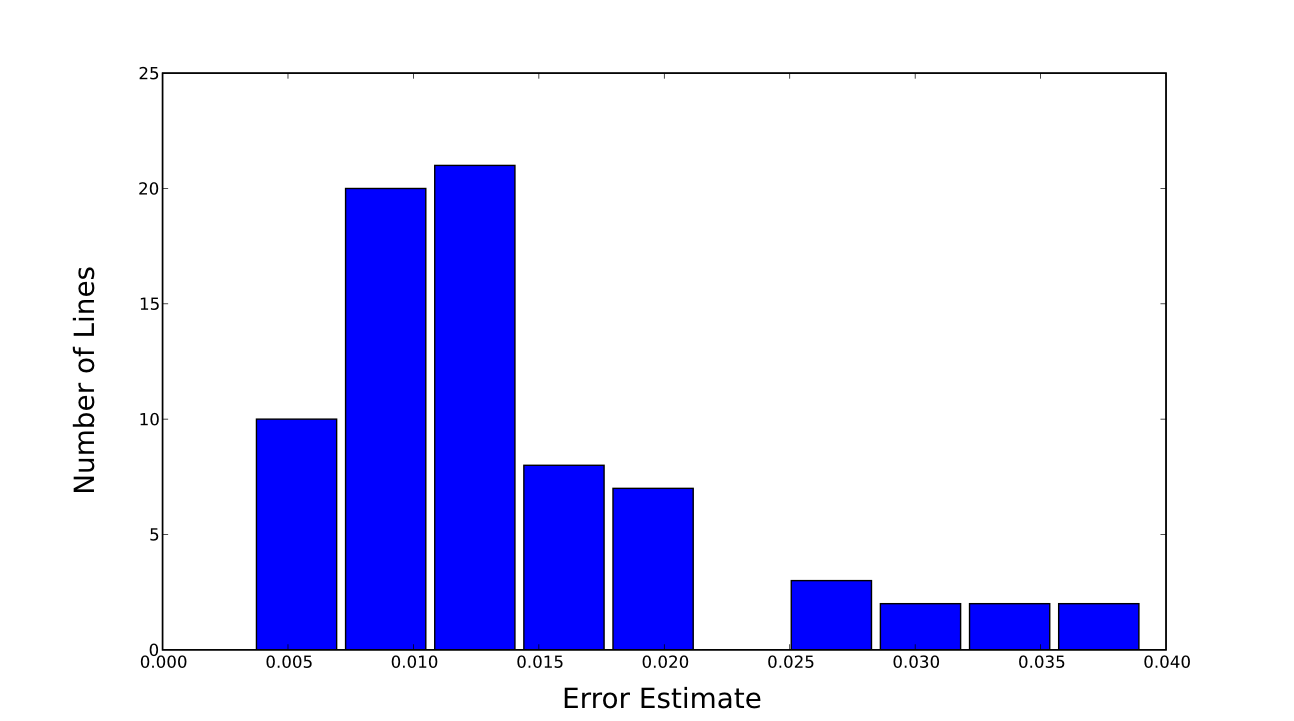
\includegraphics[width=1.0\textwidth]{figures/call_method_35_vs_2010_mismatch_rate_hist.png}
  \caption{Distribution of error estimates of 75 lines before the imputation. Average 1.396\% with standard deviation 0.00772.}\label{genotyping_f1}
\end{figure}


\begin{figure}
  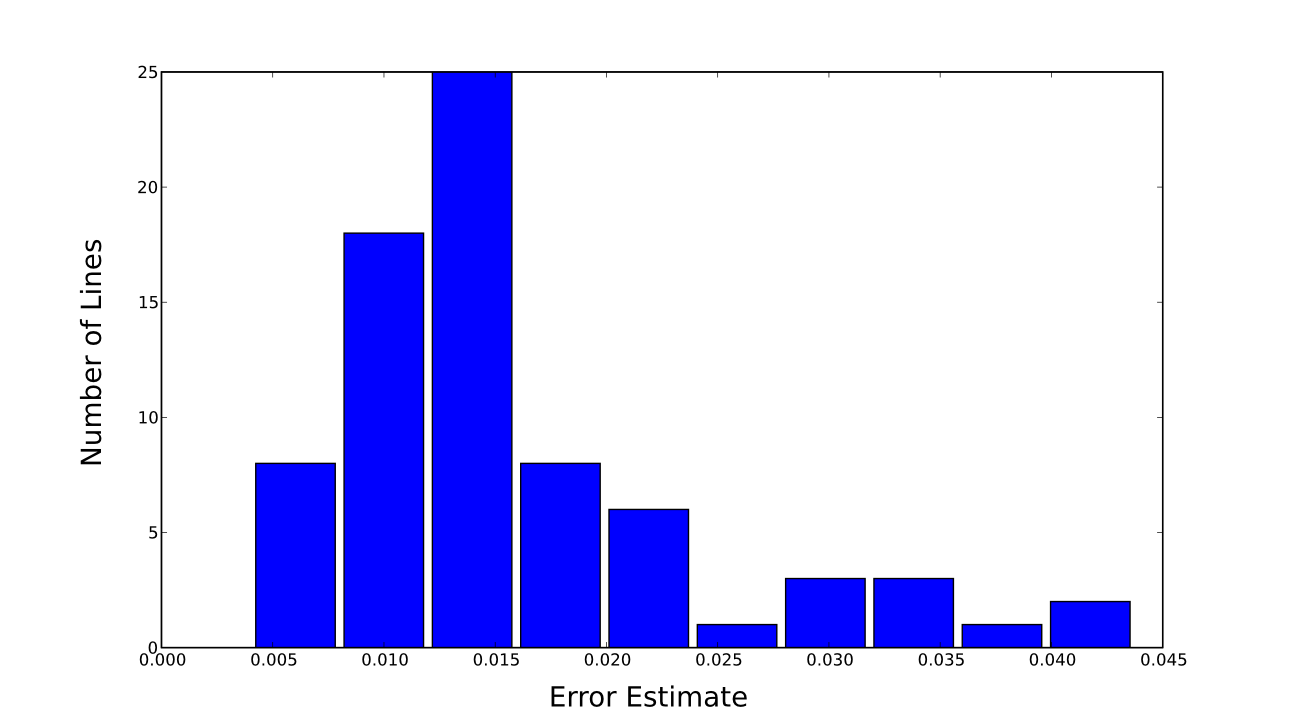
\includegraphics[width=1.0\textwidth]{figures/call_method_33_vs_2010_mismatch_rate_hist.png}
  \caption{Distribution of error estimates of 75 lines after the imputation. Average is 1.595\% with standard deviation 0.00834.}\label{genotyping_f2}
\end{figure}

\begin{figure}
  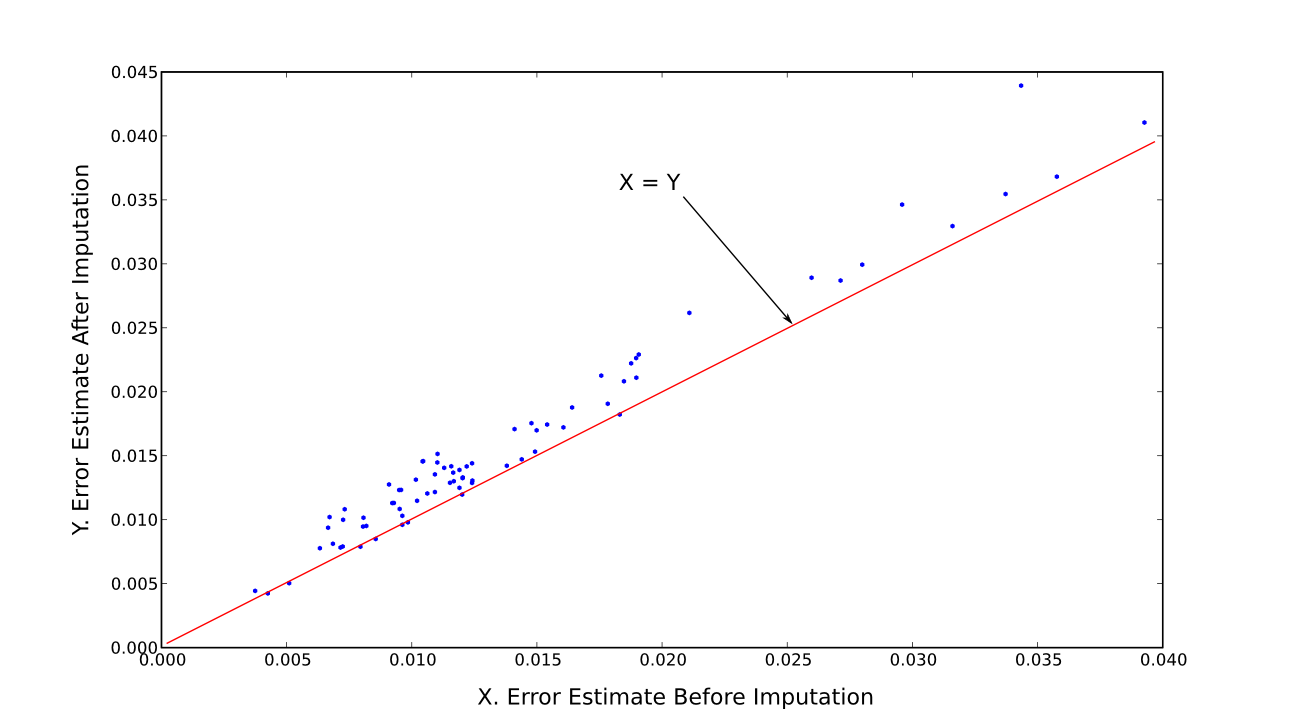
\includegraphics[width=1.0\textwidth]{figures/call_method_35_vs_2010_mismatch_rate_vs_call_method_33_vs_2010_mismatch_rate.png}
  \caption{Error estimates before the imputation (X-axis) vs. after the imputation (Y-axis). The red line denotes equality.}\label{genotyping_f3}
\end{figure}


%how many are imputed.

%how many are used to compare with 2010, mismatch rates for the imputed.

%We also have duplicates for a couple of arrays, from which we could estimate the reproducibility of our genotyping platform.


\section{Acknowledgement}
We thank B. Carvalho for his advice on how to modify the Oligo package.


\bibliography{gwa}
\bibliographystyle{apalike}

\end{document}
